The efficacy of the program was dependent on its ability to coordinate users and ensure that they were able to work together to generate the final instructions.
Thus, it was necessary to not only design an effective workflow, but to also make sure that the program implementation was easy to understand, robust, and close to the theoretical workflow.

\section{Workflow}
Turkomatic ran into difficulties in organizing the workflow. 
Their system was unable to coordinate workflows, in no small part due to the complexity of the algorithm.
Their algorithm used recursive workflow partitioning, and allowed for complex sub-task creation.
This led to significant difference of opinion between users, and little consensus was obtained without the use of a single task evaluator who would oversee the task (also known as ``derailment'' \cite{kulkarni2012collaboratively}.

To combat this problem, Canned Mentorship utilizes an iterative, one directional workflow.
Instead of a complex, largely unordered workflow of turkomatic, Canned Mentorship makes users create the instruction list in the order it will be executed.
This was done to avoid problems with granularity and starvation that were problematic in this system.

\subsection{Instruction Generation}
CannedMentorship uses a very simple task generating algorithm, with no explicit task subdivision or branching.
The system simply asks users to create steps in sequence, from beginning to end, in order.
Each step is completed in order, with the latter steps coming directly after former steps chronologically.
This avoids the issue of task subdivision. 
Users do not have to deal with the complex uncertainties of task completion, and do not have to worry about planning the task.

Previously, three-stage find, fix, verify algorithms have been used successfully in crowd-sourcing \cite{kim2013toolscape,bernstein2010soylent}. Canned Mentorship builds off of this system. 

\begin{figure}
	\begin{center}
	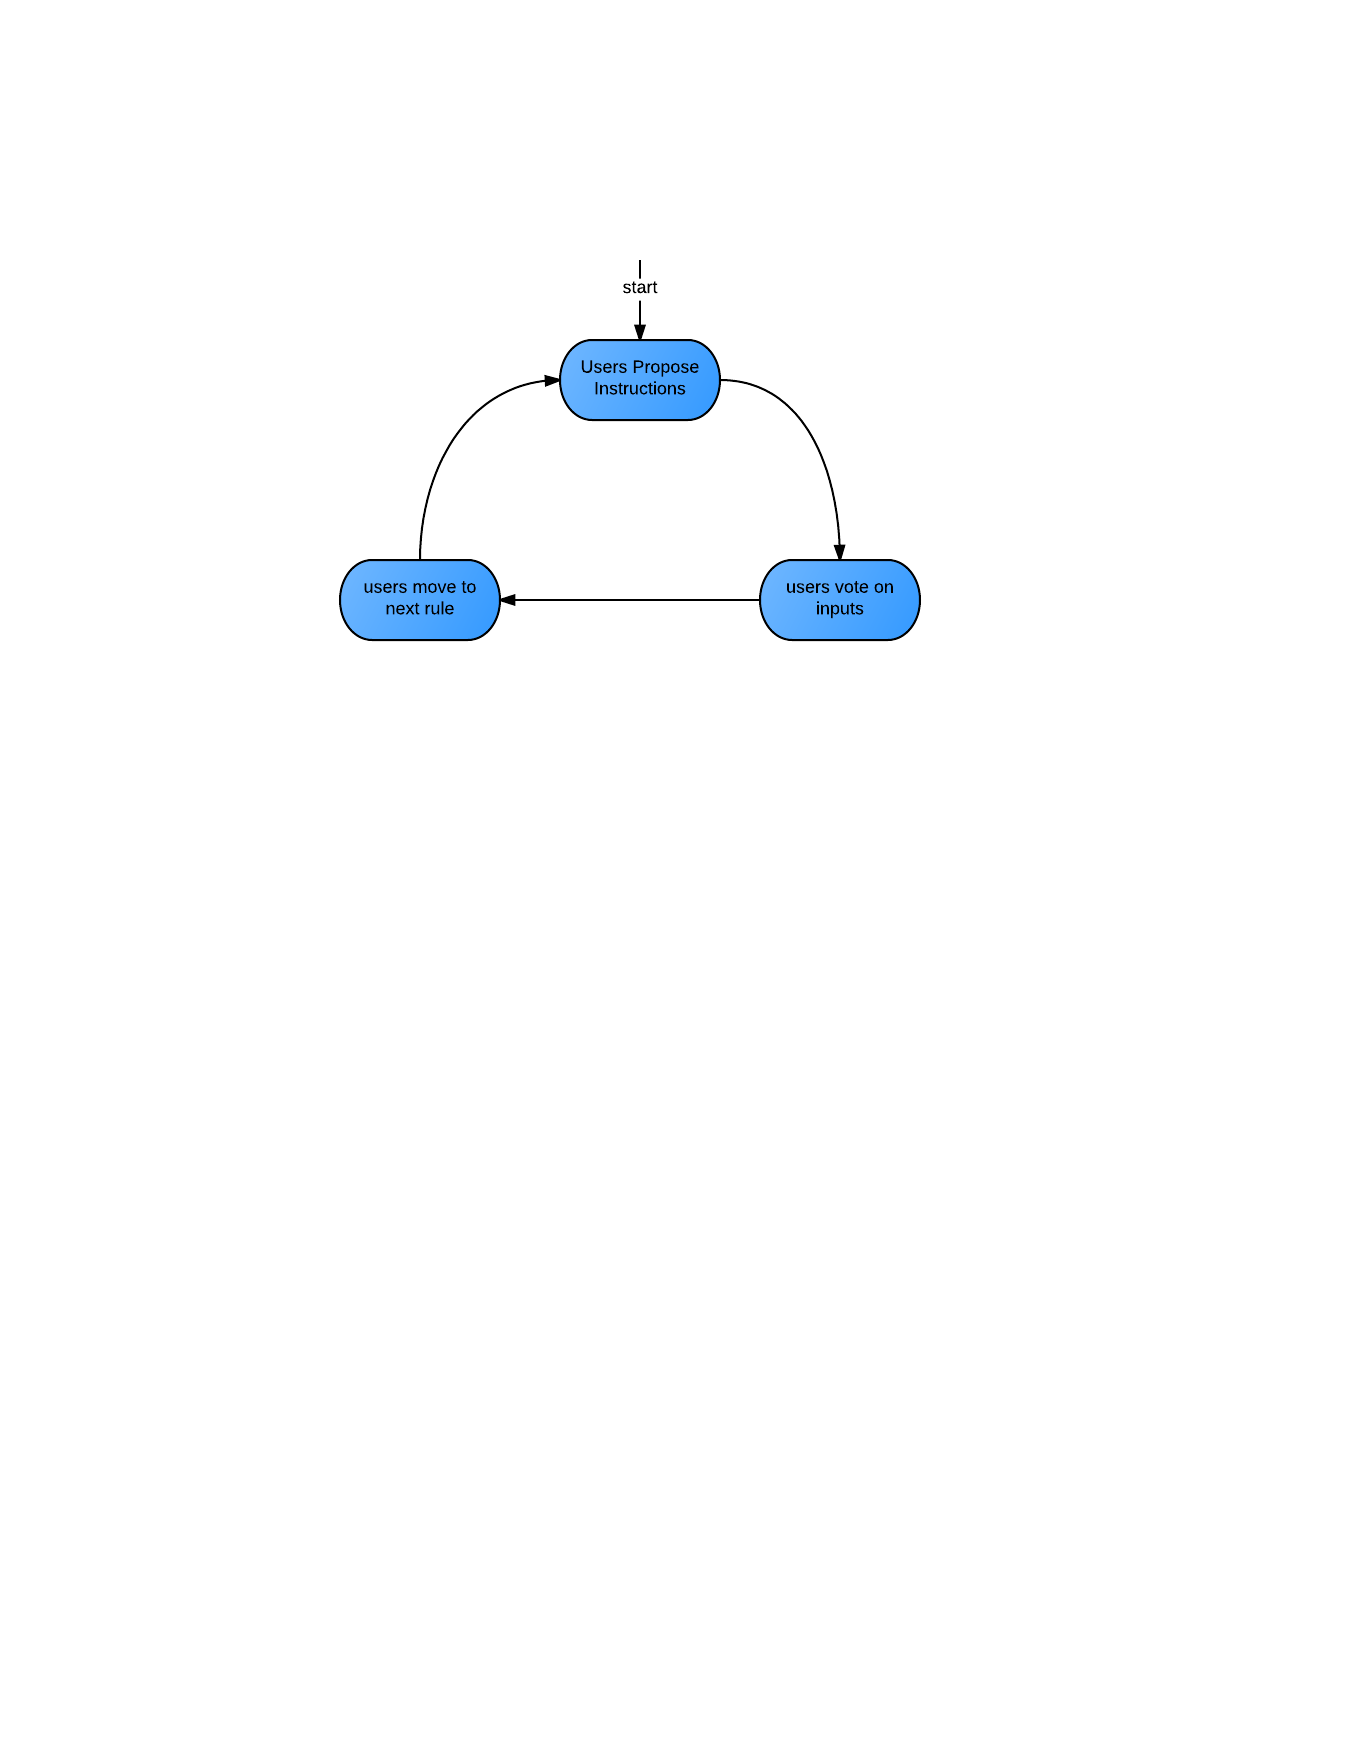
\includegraphics{figures/cmWorkflow1.png}
	\caption{The simplified version of the instruction step creation process.}
	\label{fig:cmWorkflow1}
	\end{center}
\end{figure}

In order to create an instruction step, users follow a cyclical process.
First, users suggest a step. 
Second, they vote on the available propositions.
Finally, they expand onto the next steo.
 This process for adding a new rule is illustrated with figure \ref{fig:cmWorkflow1}. 
Please note that this figure does not illustrate the overall workflow of the application, only the process for adding a new rule that users are involved in.

The ``find'' stage is already decided by the system. The users always work on the next instruction, which is the ``found'' area. 
At this point, the users are asked what the step in progress should be. 
The users type their proposition for the next instruction, which is a string of text one to two sentences in length.
The inputs are collected and compiled by the server.

At this point, the voting stage begins. 
This point, which is analogous to the ``verify'' stage noted previously, is when users select the best proposition from the group.
The instruction with the majority vote becomes the finalized instruction.

In the final step, users expand onto the next instruction. 
This step, appropriately, is similar to the ``expand'' stage employed in projects such as Soylent. 
At this stage, the instructions loop back to the beginning, and users expand the instructions by adding the next instruction that follows the newly added one.

\subsection{Additional user control}
In addition to the above, users could were also given other control flow methods. 
After an instruction was finished, and before another was started, users would be able to vote to finish the instruction set. 
If the majority voted that the current instruction set was a sufficient description for the prompt, then the task finished.

Also, Canned Mentorship implemented a ``pseudo leader'' position.
This position designated one individual to be the ``pseudo-leader'' and was given slightly more control over the rule formation than other users.
At the end of each step input from the pseudo leader was required in order to advance to the next step.
This was done to add a ``requester'' figure to the setup. 
Previous studies have shown that although users can have significant coordination and agreement difficulties when designing workflows, the presence of a leader type user with more authority over the workers can significantly improve results \cite{kulkarni2012collaboratively}.

\section{Implementation and Webapp details}
Our project began by creating a small webapp which coordinated the instruction generating process.
This program, also dubbed ``Canned Mentorship,'' consisted of two separate programs:

\begin{enumerate}
	\item a website interface for coordinating working users
	\item a back-end AI script for classifying answers and removing redundant inputs
\end{enumerate}

\section{System Implementation}

\subsection{The Webapp}
The webapp was a program written using Python Flask and was hosted on Heroku webapps. 
It was designed as a lightweight, simple system which hosted the users for the duration of the task and also coordinated their actions.

\begin{figure}[h]
	\begin{center}
		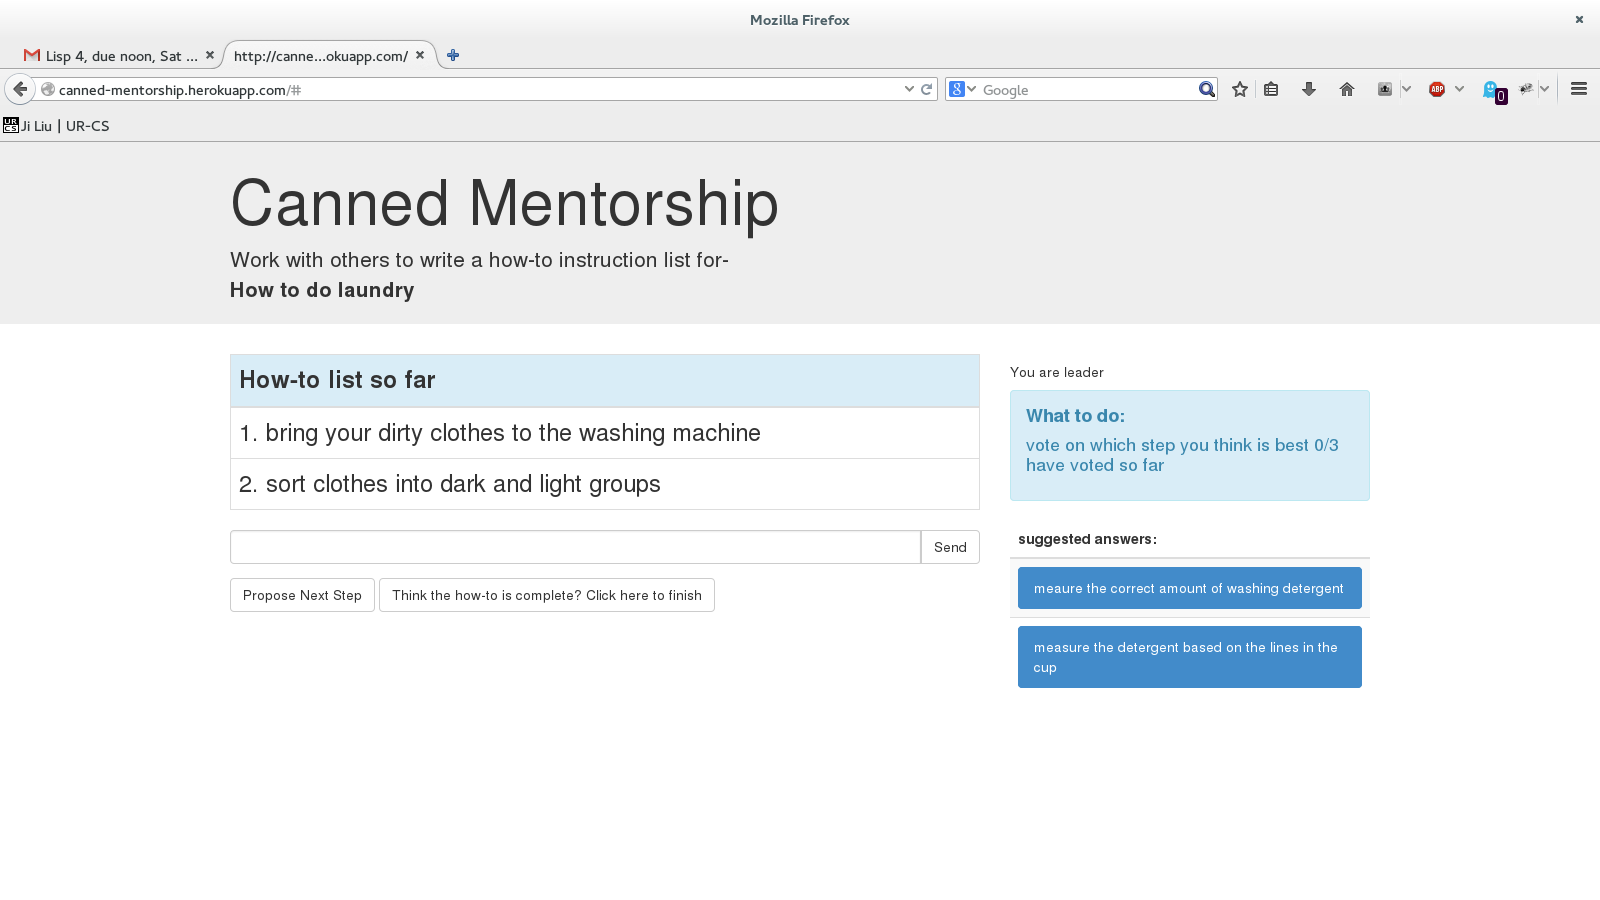
\includegraphics[width=0.48\textwidth]{figures/cmInterface.png}
		\caption{Rejection sampling was also considered as a placement mechanism.}
		\label{fig:rejection_sampling_placement}
	\end{center}
\end{figure}

As noted earlier, Heroku was chosen as the host location for the webapp ...add more stuff later...



%webapp description
%theory
%need for multiple users: john's differences
%workflow
%implementation

%ai backend
%interface with program
%parameters
	%reasons for choosing
%flow
%
\begin{comment}
\begin{figure}[h]
	\begin{center}
		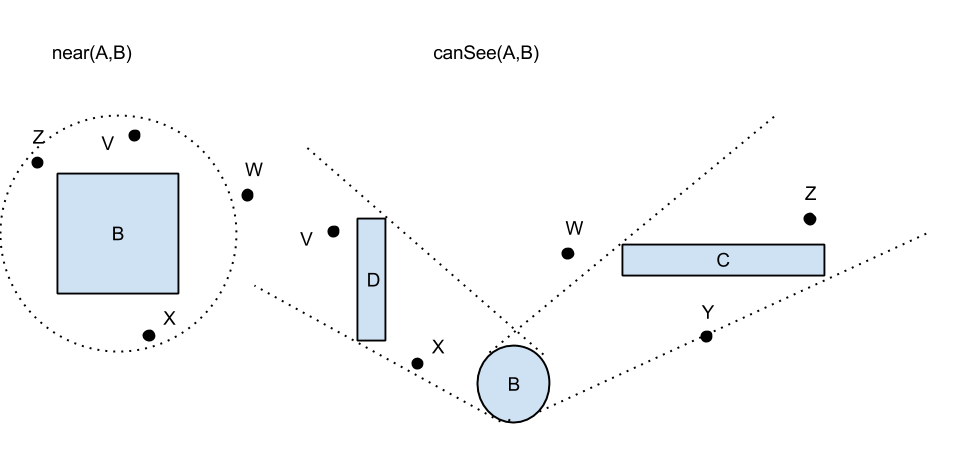
\includegraphics[width=0.48\textwidth]{figures/rejection_sampling_placement.png}
	\caption{Rejection sampling was also considered as a placement mechanism.}
	\label{fig:rejection_sampling_placement}
	\end{center}
\end{figure}
\end{comment}